\documentclass[tikz,border=5pt]{standalone}
\usepackage{tikz}
\usepackage{amsmath}
\usetikzlibrary{positioning}

\tikzset{
  tall/.style={rectangle, draw=black, thick, minimum width=0.8cm, 
               minimum height=3cm, fill=white},
  short/.style={rectangle, draw=black, thick, minimum width=0.8cm, 
                minimum height=1.5cm, fill=white},
  conn/.style={thick, black},
  dconn/.style={thick, black, dashed}
}

\begin{document}
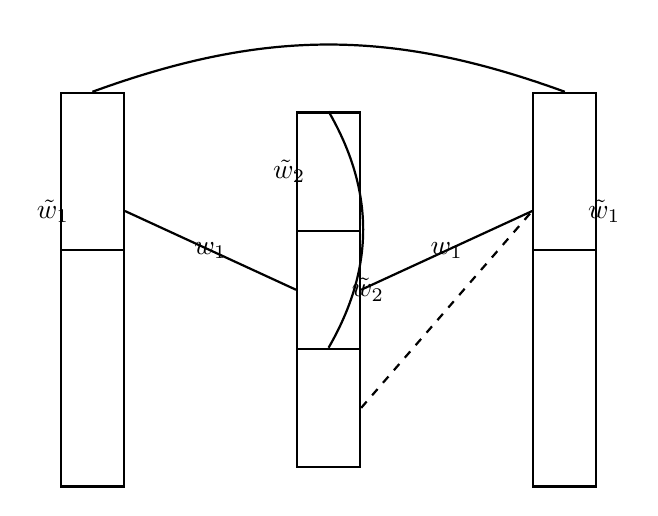
\begin{tikzpicture}[node distance=3cm and 2.5cm]
  % 左侧输入层
  \node[tall] (L1) at (0,1) {};
  \node[tall] (L2) at (0,-1) {};
  
  % 隐藏层
  \node[short] (H1) at (3,1.5) {};
  \node[short] (H2) at (3,0) {};
  \node[short] (H3) at (3,-1.5) {};
  
  % 右侧输出层
  \node[tall] (R1) at (6,1) {};
  \node[tall] (R2) at (6,-1) {};
  
  % 标签
  \node at (-0.5,1) {$\tilde{w}_1$};
  \node at (1.5,0.5) {$w_1$};
  \node at (2.5,1.5) {$\tilde{w}_2$};
  \node at (3.5,0) {$\tilde{w}_2$};
  \node at (4.5,0.5) {$w_1$};
  \node at (6.5,1) {$\tilde{w}_1$};
  
  % 连接线
  \draw[conn] (L1.east) -- (H2.west);
  \draw[conn] (H2.east) -- (R1.west);
  \draw[dconn] (H3.east) -- (R1.west);
  
  % 顶部弧线
  \draw[conn] (L1.north) to[bend left=20] (R1.north);
  \draw[conn] (H1.north) to[bend left=30] (H3.north);
\end{tikzpicture}
\end{document}